
\documentclass[letterpaper,hide notes,xcolor={table,svgnames},pdftex]{beamer}
\def\showexamples{t}


%\usepackage[svgnames]{xcolor}

%% Demo talk
%\documentclass[letterpaper,notes=show]{beamer}

\usecolortheme{crane}
\setbeamertemplate{navigation symbols}{}

\usetheme{MyPittsburgh}
%\usetheme{Frankfurt}

%\usepackage{tipa}

\usepackage{hyperref}
\usepackage{graphicx,xspace}
\usepackage[normalem]{ulem}

\newcommand\SF[1]{$\bigstar$\footnote{SF: #1}}



\newcounter{tmpnumSlide}
\newcounter{tmpnumNote}

% old question code
%\newcommand\question[1]{{$\bigstar$ \small \onlySlide{2}{#1}}}
% \newcommand\nquestion[1]{\ifdefined \presentationonly \textcircled{?} \fi \note{\par{\Large \textbf{?}} #1}}
% \newcommand\nanswer[1]{\note{\par{\Large \textbf{A}} #1}}


 \newcommand\mnote[1]{%
   \addtocounter{tmpnumSlide}{1}
   \ifdefined\showcues {~\tiny\fbox{\arabic{tmpnumSlide}}}\fi
   \note{\setlength{\parskip}{1ex}\addtocounter{tmpnumNote}{1}\textbf{\Large \arabic{tmpnumNote}:} {#1\par}}}

\newcommand\mmnote[1]{\note{\setlength{\parskip}{1ex}#1\par}}

%\newcommand\mnote[2][]{\ifdefined\handoutwithnotes {~\tiny\fbox{#1}}\fi
% \note{\setlength{\parskip}{1ex}\textbf{\Large #1:} #2\par}}

%\newcommand\mnote[2][]{{\tiny\fbox{#1}} \note{\setlength{\parskip}{1ex}\textbf{\Large #1:} #2\par}}

\newcommand\mquestion[2]{{~\color{red}\fbox{?}}\note{\setlength{\parskip}{1ex}\par{\Large \textbf{?}} #1} \note{\setlength{\parskip}{1ex}\par{\Large \textbf{A}} #2\par}\ifdefined \presentationonly \pause \fi}

\newcommand\blackboard[1]{%
\ifdefined   \showblackboard
  {#1}
  \else {\begin{center} \fbox{\colorbox{blue!30}{%
         \begin{minipage}{.95\linewidth}%
           \hspace{\stretch{1}} Some space intentionally left blank; done at the blackboard.%
         \end{minipage}}}\end{center}}%
         \fi%
}



%\newcommand\q{\tikz \node[thick,color=black,shape=circle]{?};}
%\newcommand\q{\ifdefined \presentationonly \textcircled{?} \fi}

\usepackage{listings}
\lstset{%
  keywordstyle=\bfseries,
  aboveskip=15pt,
  belowskip=15pt,
  captionpos=b,
  identifierstyle=\ttfamily,
  escapeinside={(*@}{@*)},
  stringstyle=\ttfamiliy,
  frame=lines,
  numbers=left, basicstyle=\scriptsize, numberstyle=\tiny, stepnumber=0, numbersep=2pt}

\usepackage{siunitx}
\newcommand\sius[1]{\num[group-separator = {,}]{#1}\si{\micro\second}}
\newcommand\sims[1]{\num[group-separator = {,}]{#1}\si{\milli\second}}
\newcommand\sins[1]{\num[group-separator = {,}]{#1}\si{\nano\second}}
\sisetup{group-separator = {,}, group-digits = true}

%% -------------------- tikz --------------------
\usepackage{tikz}
\usetikzlibrary{positioning}
\usetikzlibrary{arrows,backgrounds,automata,decorations.shapes,decorations.pathmorphing,decorations.markings,decorations.text}

\tikzstyle{place}=[circle,draw=blue!50,fill=blue!20,thick, inner sep=0pt,minimum size=6mm]
\tikzstyle{transition}=[rectangle,draw=black!50,fill=black!20,thick, inner sep=0pt,minimum size=4mm]

\tikzstyle{block}=[rectangle,draw=black, thick, inner sep=5pt]
\tikzstyle{bullet}=[circle,draw=black, fill=black, thin, inner sep=2pt]

\tikzstyle{pre}=[<-,shorten <=1pt,>=stealth',semithick]
\tikzstyle{post}=[->,shorten >=1pt,>=stealth',semithick]
\tikzstyle{bi}=[<->,shorten >=1pt,shorten <=1pt, >=stealth',semithick]

\tikzstyle{mut}=[-,>=stealth',semithick]

\tikzstyle{treereset}=[dashed,->, shorten >=1pt,>=stealth',thin]

\usepackage{ifmtarg}
\usepackage{xifthen}
\makeatletter
% new counter to now which frame it is within the sequence
\newcounter{multiframecounter}
% initialize buffer for previously used frame title
\gdef\lastframetitle{\textit{undefined}}
% new environment for a multi-frame
\newenvironment{multiframe}[1][]{%
\ifthenelse{\isempty{#1}}{%
% if no frame title was set via optional parameter,
% only increase sequence counter by 1
\addtocounter{multiframecounter}{1}%
}{%
% new frame title has been provided, thus
% reset sequence counter to 1 and buffer frame title for later use
\setcounter{multiframecounter}{1}%
\gdef\lastframetitle{#1}%
}%
% start conventional frame environment and
% automatically set frame title followed by sequence counter
\begin{frame}%
\frametitle{\lastframetitle~{\normalfont(\arabic{multiframecounter})}}%
}{%
\end{frame}%
}
\makeatother

\makeatletter
\newdimen\tu@tmpa%
\newdimen\ydiffl%
\newdimen\xdiffl%
\newcommand\ydiff[2]{%
    \coordinate (tmpnamea) at (#1);%
    \coordinate (tmpnameb) at (#2);%
    \pgfextracty{\tu@tmpa}{\pgfpointanchor{tmpnamea}{center}}%
    \pgfextracty{\ydiffl}{\pgfpointanchor{tmpnameb}{center}}%
    \advance\ydiffl by -\tu@tmpa%
}
\newcommand\xdiff[2]{%
    \coordinate (tmpnamea) at (#1);%
    \coordinate (tmpnameb) at (#2);%
    \pgfextractx{\tu@tmpa}{\pgfpointanchor{tmpnamea}{center}}%
    \pgfextractx{\xdiffl}{\pgfpointanchor{tmpnameb}{center}}%
    \advance\xdiffl by -\tu@tmpa%
}
\makeatother
\newcommand{\copyrightbox}[3][r]{%
\begin{tikzpicture}%
\node[inner sep=0pt,minimum size=2em](ciimage){#2};
\usefont{OT1}{phv}{n}{n}\fontsize{4}{4}\selectfont
\ydiff{ciimage.south}{ciimage.north}
\xdiff{ciimage.west}{ciimage.east}
\ifthenelse{\equal{#1}{r}}{%
\node[inner sep=0pt,right=1ex of ciimage.south east,anchor=north west,rotate=90]%
{\raggedleft\color{black!50}\parbox{\the\ydiffl}{\raggedright{}#3}};%
}{%
\ifthenelse{\equal{#1}{l}}{%
\node[inner sep=0pt,right=1ex of ciimage.south west,anchor=south west,rotate=90]%
{\raggedleft\color{black!50}\parbox{\the\ydiffl}{\raggedright{}#3}};%
}{%
\node[inner sep=0pt,below=1ex of ciimage.south west,anchor=north west]%
{\raggedleft\color{black!50}\parbox{\the\xdiffl}{\raggedright{}#3}};%
}
}
\end{tikzpicture}
}


%% --------------------

%\usepackage[excludeor]{everyhook}
%\PushPreHook{par}{\setbox0=\lastbox\llap{MUH}}\box0}

%\vspace*{\stretch{1}

%\setbox0=\lastbox \llap{\textbullet\enskip}\box0}

\setlength{\parskip}{\fill}

\newcommand\noskips{\setlength{\parskip}{1ex}}
\newcommand\doskips{\setlength{\parskip}{\fill}}

\newcommand\xx{\par\vspace*{\stretch{1}}\par}
\newcommand\xxs{\par\vspace*{2ex}\par}
\newcommand\tuple[1]{\langle #1 \rangle}
\newcommand\code[1]{{\sf \footnotesize #1}}
\newcommand\ex[1]{\uline{Example:} \ifdefined \presentationonly \pause \fi
  \ifdefined\showexamples#1\xspace\else{\uline{\hspace*{2cm}}}\fi}

\newcommand\ceil[1]{\lceil #1 \rceil}


\AtBeginSection[]
{
   \begin{frame}
       \frametitle{Outline}
       \tableofcontents[currentsection]
   \end{frame}
}



\pgfdeclarelayer{edgelayer}
\pgfdeclarelayer{nodelayer}
\pgfsetlayers{edgelayer,nodelayer,main}

\tikzstyle{none}=[inner sep=0pt]
\tikzstyle{rn}=[circle,fill=Red,draw=Black,line width=0.8 pt]
\tikzstyle{gn}=[circle,fill=Lime,draw=Black,line width=0.8 pt]
\tikzstyle{yn}=[circle,fill=Yellow,draw=Black,line width=0.8 pt]
\tikzstyle{empty}=[circle,fill=White,draw=Black]
\tikzstyle{bw} = [rectangle, draw, fill=blue!20, 
    text width=4em, text centered, rounded corners, minimum height=2em]
    
    \newcommand{\CcNote}[1]{% longname
	This work is licensed under the \textit{Creative Commons #1 3.0 License}.%
}
\newcommand{\CcImageBy}[1]{%
	\includegraphics[scale=#1]{creative_commons/cc_by_30.pdf}%
}
\newcommand{\CcImageSa}[1]{%
	\includegraphics[scale=#1]{creative_commons/cc_sa_30.pdf}%
}
\newcommand{\CcImageNc}[1]{%
	\includegraphics[scale=#1]{creative_commons/cc_nc_30.pdf}%
}
\newcommand{\CcGroupBySa}[2]{% zoom, gap
	\CcImageBy{#1}\hspace*{#2}\CcImageNc{#1}\hspace*{#2}\CcImageSa{#1}%
}
\newcommand{\CcLongnameByNcSa}{Attribution-NonCommercial-ShareAlike}

\newenvironment{changemargin}[1]{% 
  \begin{list}{}{% 
    \setlength{\topsep}{0pt}% 
    \setlength{\leftmargin}{#1}% 
    \setlength{\rightmargin}{1em}
    \setlength{\listparindent}{\parindent}% 
    \setlength{\itemindent}{\parindent}% 
    \setlength{\parsep}{\parskip}% 
  }% 
  \item[]}{\end{list}} 



\usepackage{alltt}

\title{Lecture 16 --- Testing for Android}

\author{Jeff Zarnett \& Patrick Lam \\ \small \texttt{jzarnett@uwaterloo.ca} \& \texttt{p.lam@ece.uwaterloo.ca}}
\institute{Department of Electrical and Computer Engineering \\[-1ex]
  University of Waterloo}
\date{\today}

\begin{document}

\begin{frame}
  \titlepage

  \vfill
  \begin{center}
    \CcGroupBySa{0.83}{0.95ex}\\
                  {\tiny\CcNote{\CcLongnameByNcSa}}
                  \vspace*{-2.5ex}
  \end{center}

\end{frame}

\part{Code Coverage}
\frame{\partpage}

\begin{frame}
\frametitle{Code Coverage}
\begin{changemargin}{1cm}
How well are our test cases are testing the program?

Key concept: \alert{Code Coverage}

What lines of the program are executed during our tests?

Difficult to determine when there is conditional logic.

\end{changemargin}
\end{frame}


\begin{frame}
\frametitle{Conditional Logic}
\begin{changemargin}{1cm}
Conditional: a statement evaluated to true or false.

The evaluated value is used to decide what the next step is.

Example: \texttt{if (x == 0) \{ foo(); \} else \{ bar(); \} }.

\end{changemargin}
\end{frame}

\begin{frame}
\frametitle{Coverage Definitions}
\begin{changemargin}{1cm}

There are some different definitions for coverage:
\begin{itemize}
	\item \textbf{Statement Coverage} \mnote{executing each line of code at least once;}
	\item \textbf{Branch Coverage} \mnote{traverse each branch (conditional) statement; and}
	\item \textbf{Multiple Condition Coverage} \mnote{cover all possible combinations of the conditional statements.}
\end{itemize}

\end{changemargin}
\end{frame}


\begin{frame}
\frametitle{``Covered''}
\begin{changemargin}{1cm}

A line is ``covered'' if that line is executed during the course of the test cases. 

A branch is covered if that branch is executed during the course of the test cases. 

In multiple condition coverage, a class or module is covered if all combinations of the conditionals within it are tested.
\end{changemargin}
\end{frame}


\begin{frame}
\frametitle{``Covered''}
\begin{changemargin}{1cm}
We will focus on line coverage, mostly.


Getting 100\% statement coverage is generally unrealistic.

Even if we covered all lines, we can still have bugs.

Dividing two numbers may work in the test cases. \\
\quad result in a divide by zero error if the user puts in 0. 


\end{changemargin}
\end{frame}

\begin{frame}
\frametitle{Dead Code}
\begin{changemargin}{1cm}
We say code is ``dead'' if it can never be run.

Sometimes the compiler identifies it for you.

Other times, it's only revealed by execution.

Dead code does no harm, but effort might be wasted on maintaining it.

Remove it altogether.

\end{changemargin}
\end{frame}

\begin{frame}
\frametitle{Diminishing Returns}
\begin{changemargin}{1cm}
As test cases are added we get diminishing returns.

The first test is all ``new'' lines.

Additional cases might have some overlap.

\end{changemargin}
\end{frame}

\begin{frame}
\frametitle{Case Study: EclEmma}
\begin{changemargin}{1cm}
We will examine a plug-in for Eclipse called EclEmma.

When launched, EclEmma runs the selected unit tests and then analyzes the results.

\end{changemargin}
\end{frame}

\begin{frame}
\frametitle{EclEmma Colour-Coding}
\begin{changemargin}{1cm}


EclEmma will colour-code each line in either:
\begin{itemize}
	\item \textbf{Red} -- the line was not executed;
	\item \textbf{Yellow} -- a conditional where only one branch was taken (e.g., an if was always evaluated as false); or
	\item \textbf{Green} -- the line was executed, or in the case of a conditional, both branches were taken.
\end{itemize}

\end{changemargin}
\end{frame}

\begin{frame}
\frametitle{EclEmma Colour-Coding}
\begin{center}
	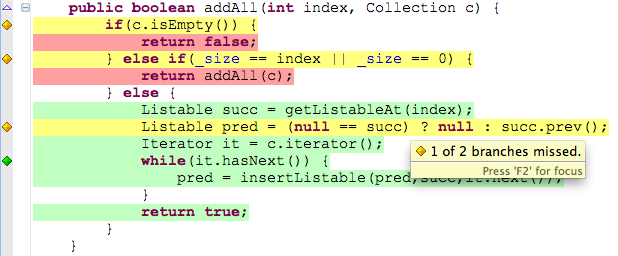
\includegraphics[width=0.75\textwidth]{images/annotations.png}
\end{center}
\end{frame}

\begin{frame}
\frametitle{EclEmma Coverage Report}
\begin{center}
	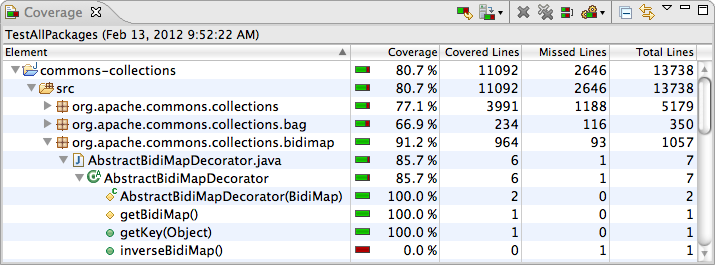
\includegraphics[width=\textwidth]{images/coverageview.png}
\end{center}
\end{frame}

\begin{frame}
\frametitle{Case Study: EclEmma}
\begin{changemargin}{1cm}
Using the coverage data, you can decide if your tests are effective in testing the logic of the code. 

Too many red lines in the project means more tests (or better tests) are needed.


\end{changemargin}
\end{frame}


\part{Testing for Android}
\frame{\partpage}

\begin{frame}
\frametitle{Avoiding Android-Specific Testing}

\begin{changemargin}{1cm}
It's easy if you test classes that don't use Android.\\[1em]

Do that, when possible.\\[1em]

Example:
\begin{itemize}
\item put step recognition code in separate class; and
\item call that code from your main Activity.
\end{itemize}
We'd be progressing towards a Model-View-Controller (ECE452) design.

\end{changemargin}
\end{frame}

\begin{frame}
\frametitle{Why Android Testing is Hard}

\begin{changemargin}{1cm}
Recall that Android apps are \structure{event-driven}.\\[1em]

Need something to produce events for you.\\[1em]

This is not really unit testing, more like integration tests.
\end{changemargin}
\end{frame}


\begin{frame}
\frametitle{What To Test\footnote{\tiny \url{http://developer.android.com/tools/testing/what_to_test.html}, accessed 7Feb13.}}

\begin{changemargin}{1cm}

Orientation change:
\begin{itemize}
\item is screen redrawn correctly?
\item did you lose any state?
\end{itemize}
~\\[0.5em]

Configuration change (e.g. adding a keyboard):
\begin{itemize}
\item again as for orientation change;
\item do you handle the new device properly?
\end{itemize}~\\[0.5em]

Battery life:
\begin{itemize}
\item don't hog the battery (out of scope for us).
\end{itemize}~\\[0.5em]

External resources:
\begin{itemize}
\item how does your app behave when it doesn't have
necessary resources, e.g. GPS?
\end{itemize}

\end{changemargin}

\end{frame}

\begin{frame}
\frametitle{Android Activity Unit Tests}

\begin{changemargin}{1cm}
\large
This is allegedly possible using {\tt ActivityUnitTestCase}.\\[1em]
More like unit tests than what we'll see next.\\[1em]
There is no useful documentation on the Internet, apart from Javadoc.\\[1em]
Beyond the scope of this course.
\end{changemargin}
\end{frame}



\part{Case Study: QA for Android Games}
\frame{\partpage}

\begin{frame}
\frametitle{Android Game Testing}
\begin{changemargin}{1cm}

Now we will examine a real situation: Android Game Testing

\begin{center}
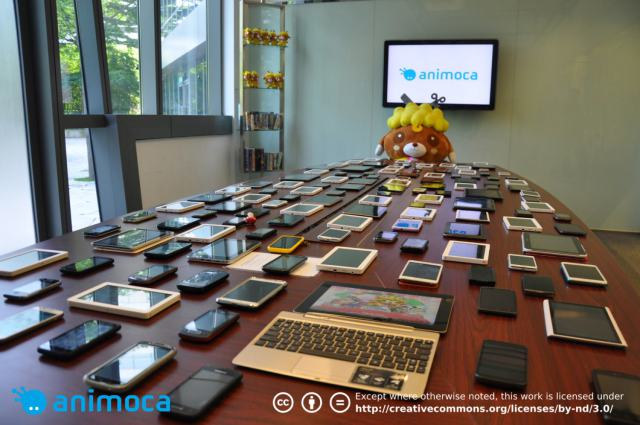
\includegraphics[width=0.75\textwidth]{images/androiddevices.jpg}
\end{center}

\end{changemargin}
\end{frame}


\begin{frame}
\frametitle{Android Games: Challenge}
\begin{changemargin}{1cm}

The biggest challenge is: fragmentation. \mnote{there are literally hundreds of different devices out there, made by different manufacturers, with different specifications. A Hong Kong developer, Animoca, tests on about 400 different phones and tablets. This is a lot, but this is easy in comparison to the era of what were called ``feature phones'' -- when just about every phone was unique. Android provides at least \emph{some} standardization.}


\begin{center}
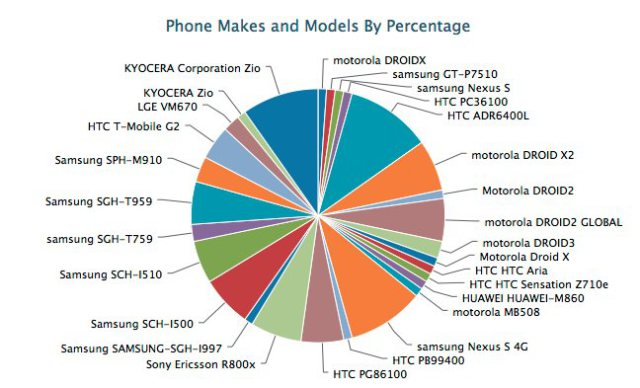
\includegraphics[width=0.9\textwidth]{images/android-install.jpeg}
\end{center}

\end{changemargin}
\end{frame}

\begin{frame}
\frametitle{Android Game Testing}
\begin{changemargin}{1cm}

Tip 1: \textbf{Test on Real Devices}.

Emulators are good, but not perfect.

Sensors and touch interface hard to emulate.

\end{changemargin}
\end{frame}

\begin{frame}
\frametitle{Android Game Testing}
\begin{changemargin}{1cm}

Tip 2: \textbf{Choose your Devices}.

How many is enough? \\
\quad Some use a small number (5-12); others $>$ 40.

Criteria: phone vs tablet, highres vs lowres screen, GPU.

Individual devices (e.g., Galaxy S3).

\end{changemargin}
\end{frame}

\begin{frame}
\frametitle{Android Game Testing}
\begin{changemargin}{1cm}

Tip 3: \textbf{Know what NOT to test}.

Decide what devices you will not support.

Choose to say no to small, slow, or outdated devices. \mnote{port. You may choose to say no to small, slow, or outdated phones and operating systems. It will not be possible to support every single Android device in the world, so focus your testing effort where it gets the most ``bang for the buck''. It's often better to choose not to support a low-end device (or old OS) than it is to test your app on a phone that's owned by 4 people in the world (or worse... release your software untested).}

\end{changemargin}
\end{frame}

\begin{frame}
\frametitle{Android Game Testing}
\begin{changemargin}{1cm}

Tip 4: \textbf{Test Continuously}.

Pocket Gems creates test, but offshore the rest of the testing.

The offshore team files bugs.

Tests created concurrently with development.

\end{changemargin}
\end{frame}

\begin{frame}
\frametitle{Android Game Testing: Lessons}
\begin{changemargin}{1cm}

It's not enough to just check the software.\\
	\quad Battery life, memory use, and performance must be tested.

Testing is tightly integrated - no ``big bang'' testing.

Run a final, extra thorough test phase before release.

\end{changemargin}
\end{frame}

\end{document}
